\documentclass[12pt]{extarticle}
\usepackage[utf8]{inputenc}
\usepackage{graphicx}
\usepackage{float}

% Disable indentation
\setlength{\parindent}{0pt}

\title{Lab: Remote Method Invocation}
\author{Alexander Hoffmann}
\date{\today}

\begin{document}

\maketitle

RMI stands for Remote Method Invocation. It is a mechanism that allows an object residing in one system (JVM) to access/invoke an object running on another JVM. RMI is used to build distributed applications; it provides remote communication between Java programs.

\section{Local execution}
\textbf{Q1.} The package contains three main methods in \texttt{Registry.java}, \texttt{Server.java} and \texttt{Client.java}.

\textbf{Q2.} The Java processes will be executed until terminated manually. This means, even if the main methods of each and every class is done, the processes will keep on running.

\textbf{Q3.} First, run \texttt{Registry.java} as is it referenced in \texttt{Server.java}. Next, run \texttt{Server.java}. Finally, run \texttt{Client.java}.

\textbf{Q4.} If we run \texttt{Registry.java} alone, everything works as it should because this is the process to execute first. Now suppose we run \texttt{Server.java} alone. We are getting an error. The console states that the hostname is undefined. This is because the host is initialized in the Registry class. Finally, if we try to execute \texttt{Client.java} independently, this app crashes as the local server cannot send the \texttt{Object} to the client.

\textbf{Q5.} 1. Suppose we launch \texttt{Registry.java}, then \texttt{Server.java} and stop \texttt{Registry.java}. Now if we run \texttt{Client.java}, the process crashes because of a \texttt{ConnectionRefused} exception.\\
2. Now \texttt{Registry.java} has been restarted. We try to run \texttt{Client.java} but it crashes because of an \texttt{NotBoundException}. The server has to rebind with the new registry.\\
3. Restart the server which will now bind. If we run the client now, it works fine.\\
4. Finally, restart the server and try again to launch the client. It works.

\textbf{Q6.} The client needs the server which needs to bind to the registry. The client is direclty dependent of the server and indirectly dependent of the registry. The server directly depends on the registry. The registry is completely independent.

\section{Distributed execution}
\textbf{Q1.} The server side classes should be deployed on one machine whereas the client side classes should be executed on the other machine.

\textbf{Q2.} \texttt{Registry.java}, \texttt{Server.java}, \texttt{Sorter.java} and \texttt{SimpleSorter.java} are stored on the server machine. \texttt{Client.java} is executed on the client machine.

\textbf{Q3.} Since we are not running the server locally anymore, we need to change the IP address of the server to be accessible by the other machine on the network.

\textbf{Q4.} We create a virtual machine running an Ubuntu server where we deploy the server side of the application. Here is the file structure on the server.
\begin{center}
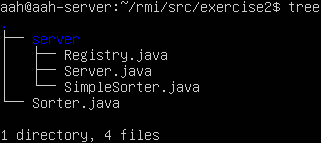
\includegraphics[scale=0.7]{resources/2-4-1.png}
\end{center}
On the client, change the IP address in the constant \texttt{SERVICE\_HOST} to \texttt{192.168.1.76} which corresponds to the IP address of the server.

After all is set and done, run \texttt{Registry.java} on the server.
\begin{center}
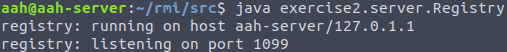
\includegraphics[scale=0.7]{resources/2-4-3.png}
\end{center}
And \texttt{Server.java}. Then run \texttt{Client.java} on the host. Here is the output on the console of the server.
\begin{center}
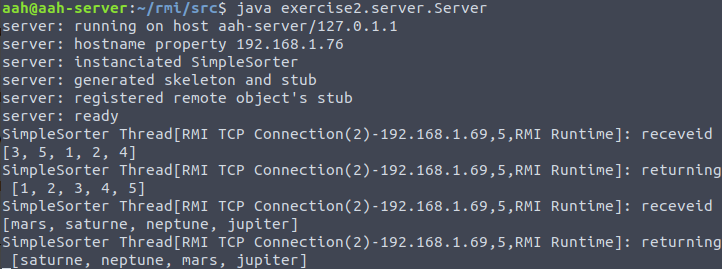
\includegraphics[scale=0.5]{resources/2-4-2.png}
\end{center}

The rest of the lab is described in the source code provided in the compressed folder.

\end{document}
